% ============================================================
%  Referat APD2 — UPB ETTI
%  Identificarea Similaritatilor intre Documente cu Python MPI
% ============================================================
\documentclass[a4paper,12pt]{report}

% --- Encoding & Language ---
\usepackage[T1]{fontenc}
\usepackage[utf8]{inputenc}
\usepackage[romanian]{babel}

% --- Page geometry (UPB standard) ---
\usepackage[a4paper, top=2.5cm, bottom=2.5cm, left=3cm, right=2.5cm]{geometry}

% --- Fonts ---
\usepackage{mathptmx}        % Times New Roman
\usepackage{microtype}

% --- Line spacing ---
\usepackage{setspace}
\onehalfspacing

% --- Graphics & Floats ---
\usepackage{graphicx}
\usepackage{float}
\usepackage{caption}
\usepackage{subcaption}

% --- Math ---
\usepackage{amsmath, amssymb}

% --- Tables ---
\usepackage{booktabs}
\usepackage{array}

% --- Code listings ---
\usepackage{listings}
\usepackage{xcolor}
\lstset{
  basicstyle=\ttfamily\small,
  keywordstyle=\color{blue}\bfseries,
  commentstyle=\color{gray},
  stringstyle=\color{teal},
  breaklines=true,
  frame=single,
  numbers=left,
  numberstyle=\tiny\color{gray},
  tabsize=4,
  showstringspaces=false,
  language=Python
}

% --- Acronyms ---
\usepackage{acronym}

% --- Diagrams ---
\usepackage{tikz}
\usetikzlibrary{shapes.geometric, arrows.meta, positioning, fit, backgrounds}

% --- Header / Footer ---
\usepackage{fancyhdr}
\pagestyle{fancy}
\fancyhf{}
\fancyhead[L]{\small\leftmark}
\fancyhead[R]{\small\thepage}
\renewcommand{\headrulewidth}{0.4pt}

% --- Hyperlinks ---
\usepackage[hidelinks, unicode]{hyperref}

% --- Indent first paragraph ---
\usepackage{indentfirst}
\setlength{\parindent}{1.25cm}

% --- Chapter title style ---
\usepackage{titlesec}
\titleformat{\chapter}[block]{\normalfont\large\bfseries\centering}{CAPITOLUL \thechapter.}{0.5em}{\MakeUppercase}
\titlespacing*{\chapter}{0pt}{-10pt}{20pt}

% ============================================================
%  Metadata
% ============================================================
\newcommand{\univname}{Universitatea Politehnica din Bucure\c{s}ti}
\newcommand{\facname}{Facultatea de Electronic\u{a}, Telecomunica\c{t}ii \c{s}i\\Tehnologia Informa\c{t}iei}
\newcommand{\deptname}{Departamentul de Telecomunica\c{t}ii \c{s}i Tehnologia Informa\c{t}iei}
\newcommand{\coursename}{Algoritmi Paraleli \c{s}i Distribui\c{t}i}
\newcommand{\titlul}{Identificarea Similari\c{t}\u{a}\c{t}ilor \^{i}ntre Documente\\folosind Python MPI (mpi4py)}
\newcommand{\studentone}{[Prenume NUME Student 1]}
\newcommand{\studenttwo}{[Prenume NUME Student 2]}
\newcommand{\grupaname}{[Grupa XXX]}
\newcommand{\anuniv}{2025 -- 2026}

% ============================================================
\begin{document}

% ============================================================
%  COPERTA (Pagina de titlu)
% ============================================================
\begin{titlepage}
  \centering
  \vspace*{0.5cm}

  {\large\bfseries \univname}\\[0.3cm]
  {\large \facname}\\[0.1cm]
  {\normalsize \deptname}\\[1.5cm]

  \rule{\linewidth}{0.5mm}\\[0.4cm]
  {\LARGE\bfseries \titlul}\\[0.4cm]
  \rule{\linewidth}{0.5mm}\\[1.5cm]

  {\large \textbf{Disciplina:} \coursename}\\[2.5cm]

  \begin{center}
    \large
    \textbf{Studen\c{t}i:}\\[0.4cm]
    \studentone\\[0.15cm]
    \studenttwo\\[0.15cm]
    \grupaname
  \end{center}

  \vfill
  {\large Bucure\c{s}ti, \anuniv}
\end{titlepage}

% ============================================================
%  LISTA FIGURILOR
% ============================================================
\listoffigures
\addcontentsline{toc}{chapter}{Lista Figurilor}
\newpage

% ============================================================
%  LISTA ACRONIMELOR
% ============================================================
\chapter*{Lista Acronimelor}
\addcontentsline{toc}{chapter}{Lista Acronimelor}

\begin{acronym}[MSMPI]
  \acro{MPI}{Message Passing Interface}
  \acro{HPC}{High-Performance Computing}
  \acro{LSH}{Locality-Sensitive Hashing}
  \acro{TF-IDF}{Term Frequency -- Inverse Document Frequency}
  \acro{NLP}{Natural Language Processing}
  \acro{API}{Application Programming Interface}
  \acro{CPU}{Central Processing Unit}
  \acro{RAM}{Random Access Memory}
  \acro{PDF}{Portable Document Format}
  \acro{HTML}{HyperText Markup Language}
  \acro{BLAS}{Basic Linear Algebra Subprograms}
  \acro{MSMPI}{Microsoft MPI}
\end{acronym}
\newpage

% ============================================================
%  CUPRINS
% ============================================================
\tableofcontents
\newpage

% ============================================================
\chapter{Enun\c{t}ul Temei}
% ============================================================

Tema de fa\c{t}\u{a} face parte din domeniul algoritmilor paraleli \c{s}i distribui\c{t}i aplica\c{t}i asupra problemelor de prelucrare a textului la scar\u{a} mare. Enun\c{t}ul complet al temei este:

\begin{quote}
\textit{Implementa\c{t}i un sistem distribuit pentru identificarea perechilor celor mai similare documente dintr-un corpus de dimensiuni mari. Sistemul trebuie s\u{a} utilizeze paradigma Master-Worker cu \texttt{mpi4py}, s\u{a} accepte documente \^{i}n formate eterogene (PDF, TXT, HTML) \c{s}i s\u{a} aplice tehnici de reducere a complexit\u{a}\c{t}ii (MinHash/LSH) pentru a evita compararea na\"{\i}v\u{a} $\mathcal{O}(N^2)$.}
\end{quote}

\section{Date de intrare}

Sistemul accept\u{a} ca date de intrare un num\u{a}r arbitrar de documente \^{i}n formate diferite:
\begin{itemize}
  \item Fi\c{s}iere text simplu (\texttt{.txt})
  \item Documente \ac{PDF} (extrase cu \texttt{pdfplumber})
  \item Pagini web \texttt{.html}/\texttt{.htm} (parsate cu \texttt{BeautifulSoup4})
  \item Colec\c{t}ii publice (datasetul \texttt{20newsgroups} din \texttt{scikit-learn})
  \item Date sintetice generate procedural pentru benchmark
\end{itemize}

\section{Date de ie\c{s}ire}

Sistemul returneaz\u{a} un top-$N$ al celor mai similare perechi de documente, unde fiecare intrare con\c{t}ine:
\begin{itemize}
  \item Identificatorii celor dou\u{a} documente
  \item Scorul de similaritate cosinus (valoare \^{i}n intervalul $[0, 1]$)
\end{itemize}

\section{Parametri de configurare}

Sistemul accept\u{a} urm\u{a}torii parametri prin linia de comand\u{a}:
\begin{itemize}
  \item \texttt{--docs $N$} — num\u{a}rul de documente prelucrate
  \item \texttt{--chunk-size $C$} — num\u{a}rul de r\^{a}nduri per task distribuit workerilor
  \item \texttt{--top-n $K$} — num\u{a}rul de perechi returnate \^{i}n rezultat
  \item \texttt{--source \{newsgroups, synthetic, files, db\}} — sursa documentelor
\end{itemize}

% ============================================================
\chapter{Context \c{s}i Motiva\c{t}ie}
% ============================================================

\section{Importan\c{t}a problemei}

Identificarea similarit\u{a}\c{t}ilor dintre documente reprezint\u{a} o problem\u{a} fundamental\u{a} \^{i}n \ac{NLP} \c{s}i \^{i}n sistemele de regasire a informa\c{t}iei. Aplica\c{t}iile practice sunt numeroase:

\begin{itemize}
  \item \textbf{Detec\c{t}ia plagiatului} — compararea lucr\u{a}rilor academice sau a codului surs\u{a} pentru identificarea copierilor
  \item \textbf{Deduplicarea con\c{t}inutului web} — motoarele de c\u{a}utare (Google, Bing) eliminau miliarde de pagini duplicate \^{i}nc\u{a} din 2003
  \item \textbf{Sisteme de recomandare} — g\u{a}sirea articolelor, produselor sau filmelor similare cu un element dat
  \item \textbf{Clustering de documente} — gruparea automat\u{a} a \c{s}tirilor, documentelor juridice sau rapoartelor medicale
  \item \textbf{Detec\c{t}ia informa\c{t}iilor false} — identificarea variantelor aceluia\c{s}i articol modificat u\c{s}or
\end{itemize}

\section{Provocarea scalabilit\u{a}\c{t}ii}

Abordarea na\"{\i}v\u{a} a problemei implic\u{a} compararea tuturor perechilor posibile din corpus. Pentru un set de $N$ documente, num\u{a}rul de perechi este:
\begin{equation}
  \binom{N}{2} = \frac{N(N-1)}{2} \approx \frac{N^2}{2}
\label{eq:naive}
\end{equation}

La 10.000 de documente, rezult\u{a} aproximativ 50 de milioane de compara\c{t}ii. La 1 milion de documente (dimensiunea unui motor de c\u{a}utare mic), rezult\u{a} $5 \times 10^{11}$ opera\c{t}ii — imposibil de realizat secven\c{t}ial \^{i}ntr-un timp rezonabil.

Aceast\u{a} cre\c{s}tere p\u{a}tratic\u{a} a complexit\u{a}\c{t}ii justific\u{a} necesitatea a dou\u{a} m\u{a}suri complementare:
\begin{enumerate}
  \item \textbf{Reducerea algoritmice} — tehnici de indexare aproximativ\u{a} (LSH) care reduc num\u{a}rul de compara\c{t}ii necesare
  \item \textbf{Paralelizarea} — distribuirea computa\c{t}iei pe mai multe procese/noduri
\end{enumerate}

% ============================================================
\chapter{Fundamente Teoretice \c{s}i Istoric}
% ============================================================

\section{Reprezentarea textului — \ac{TF-IDF}}

Introdus\u{a} de Salton \c{s}i McGill \^{i}n 1983 \cite{salton1983}, metoda \ac{TF-IDF} transform\u{a} documentele text \^{i}n vectori numerici din spa\c{t}iul termenilor. Greutatea unui termen $t$ \^{i}ntr-un document $d$ este:

\begin{equation}
  \text{TF-IDF}(t,d) = \text{TF}(t,d) \cdot \text{IDF}(t)
  = \left(1 + \log f_{t,d}\right) \cdot \log\!\frac{N}{n_t}
\label{eq:tfidf}
\end{equation}

unde $f_{t,d}$ este frecven\c{t}a termenului $t$ \^{i}n documentul $d$, $N$ este num\u{a}rul total de documente, iar $n_t$ este num\u{a}rul de documente care con\c{t}in termenul $t$.

\section{Similaritatea Cosinus}

Dou\u{a} documente reprezentate ca vectori TF-IDF $\mathbf{a}$ \c{s}i $\mathbf{b}$ sunt comparate prin similaritatatea cosinus:

\begin{equation}
  \text{sim}(\mathbf{a}, \mathbf{b}) = \cos\theta = \frac{\mathbf{a} \cdot \mathbf{b}}{\|\mathbf{a}\|\,\|\mathbf{b}\|}
\label{eq:cosine}
\end{equation}

Valorile sunt \^{i}n intervalul $[0, 1]$ pentru vectori nenegativi: $0$ indic\u{a} documente complet diferite, $1$ indic\u{a} documente identice.

\section{MinHash \c{s}i Similaritatea Jaccard}

Similaritatea Jaccard m\u{a}soar\u{a} suprapunerea dintre dou\u{a} mul\c{t}imi:
\begin{equation}
  J(A,B) = \frac{|A \cap B|}{|A \cup B|}
\label{eq:jaccard}
\end{equation}

Algoritmul \textbf{MinHash}, propus de Broder \^{i}n 1997 \cite{broder1997}, estimeaz\u{a} eficient similaritatea Jaccard. Pentru o familie de func\c{t}ii hash $\{h_k\}_{k=1}^{K}$, semnatura MinHash a unui document $D$ este:
\begin{equation}
  \text{sig}(D) = \left[\min_{t \in D} h_1(t),\; \min_{t \in D} h_2(t),\; \ldots,\; \min_{t \in D} h_K(t)\right]
\label{eq:minhash}
\end{equation}

Proprietatea fundamental\u{a} este:
\begin{equation}
  \Pr\!\left[h_k(D_1) = h_k(D_2)\right] = J(D_1, D_2)
\label{eq:minhash_prob}
\end{equation}

Cu $K = 128$ func\c{t}ii hash, eroarea de estimare este $\sigma \approx 1/\sqrt{K} \approx 0.088$.

\section{Locality-Sensitive Hashing (LSH)}

Tehnica \ac{LSH}, introdus\u{a} de Indyk \c{s}i Motwani \^{i}n 1998 \cite{indyk1998}, utilizeaz\u{a} semn\u{a}turile MinHash pentru a g\u{a}si perechi similare f\u{a}r\u{a} a compara toate perechile. Matricea de semn\u{a}turi (shape: $N \times K$) este \^{i}mp\u{a}r\c{t}it\u{a} \^{i}n $b$ benzi de c\^{a}te $r = K/b$ r\^{a}nduri fiecare.

Dou\u{a} documente devin \textit{candidat\c{t}i} dac\u{a} colidez\u{a} \^{i}n cel pu\c{t}in o band\u{a} (semn\u{a}turile lor sunt identice \^{i}n to\c{t}i cei $r$ indici ai benzii). Probabilitatea ca o pereche cu similaritate Jaccard $s$ s\u{a} fie detectat\u{a} este:
\begin{equation}
  P(\text{candidat} \mid J = s) = 1 - (1 - s^r)^b
\label{eq:lsh_prob}
\end{equation}

Pentru $K=128$, $b=16$, $r=8$, pragul de detec\c{t}ie (probabilitate 50\%) este $s^* \approx 0.55$.

\section{MPI — Message Passing Interface}

Standardul \ac{MPI} a ap\u{a}rut \^{i}n 1994, definind o interfa\c{t}\u{a} portabil\u{a} de comunicare \^{i}ntre procese paralele. Versiunea 3.1 (2015) r\u{a}m\^{a}ne standardul dominant \^{i}n \ac{HPC}. Principalele primitive utilizate \^{i}n aceast\u{a} lucrare sunt:
\begin{itemize}
  \item \texttt{MPI\_Bcast} — difuzarea unui buffer c\u{a}tre toate procesele (zero-copy pentru NumPy)
  \item \texttt{MPI\_Send} / \texttt{MPI\_Recv} — trimitere/primire punct-la-punct cu buffer explicit
  \item \texttt{MPI\_ANY\_SOURCE} — primire de la orice proces disponibil (baza load balancing-ului dinamic)
\end{itemize}

Biblioteca \texttt{mpi4py} \cite{dalcin2011} expune \ac{MPI} \^{i}n Python. Func\c{t}iile cu liter\u{a} mare (\texttt{comm.Send}, \texttt{comm.Recv}, \texttt{comm.Bcast}) accept\u{a} buffere NumPy direct, evit\^{a}nd serializarea pickle specific\u{a} variantelor cu liter\u{a} mic\u{a}.

% ============================================================
\chapter{Arhitectura Solu\c{t}iei}
% ============================================================

\section{Pipeline general}

Sistemul implementat urmeaz\u{a} un pipeline \^{i}n patru faze:

\begin{enumerate}
  \item \textbf{Preprocesare} — extragerea textului din documente eterogene
  \item \textbf{Vectorizare} — calculul matricei TF-IDF
  \item \textbf{Generare candida\c{t}i} — identificarea perechilor probabil similare cu MinHash + LSH
  \item \textbf{Calcul distribuit} — calculul similarit\u{a}\c{t}ii cosinus \^{i}ntre candida\c{t}i, distribuit \^{i}n paradigma Master-Worker
\end{enumerate}

\section{Paradigma Master-Worker cu Load Balancing Dinamic}

\begin{figure}[H]
\centering
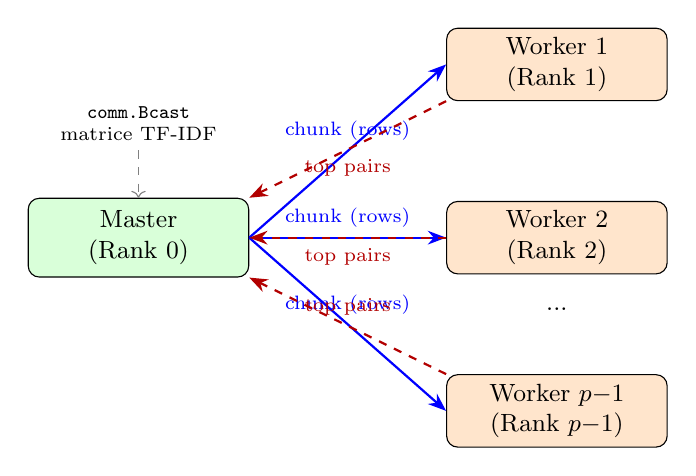
\begin{tikzpicture}[
  node distance = 1.2cm and 2.5cm,
  box/.style   = {rectangle, rounded corners, draw, fill=blue!10,
                  minimum width=2.8cm, minimum height=1cm, align=center, font=\small},
  worker/.style= {rectangle, rounded corners, draw, fill=orange!20,
                  minimum width=2.8cm, minimum height=0.9cm, align=center, font=\small},
  arr/.style   = {-Stealth, thick}
]

\node[box, fill=green!15] (master) {Master\\(Rank 0)};
\node[worker, right=of master, yshift= 2.2cm] (w1) {Worker 1\\(Rank 1)};
\node[worker, right=of master]                (w2) {Worker 2\\(Rank 2)};
\node[worker, right=of master, yshift=-2.2cm] (w3) {Worker $p{-}1$\\(Rank $p{-}1$)};
\node[font=\small, below=0.3cm of w2] {...};

% Arrows master -> workers
\draw[arr, blue] (master.east) -- node[above, font=\scriptsize]{chunk (rows)} (w1.west);
\draw[arr, blue] (master.east) -- node[above, font=\scriptsize]{chunk (rows)} (w2.west);
\draw[arr, blue] (master.east) -- node[above, font=\scriptsize]{chunk (rows)} (w3.west);

% Arrows workers -> master (results)
\draw[arr, red!70!black, dashed] (w1.south west) -- node[below, font=\scriptsize]{top pairs} (master.north east);
\draw[arr, red!70!black, dashed] (w2.west)        -- node[below, font=\scriptsize]{top pairs} (master.east);
\draw[arr, red!70!black, dashed] (w3.north west)  -- node[above, font=\scriptsize]{top pairs} (master.south east);

% Bcast label
\node[above=0.6cm of master, font=\scriptsize, align=center] (bcast) {\texttt{comm.Bcast}\\matrice TF-IDF};
\draw[->, dashed, gray] (bcast) -- (master);

\end{tikzpicture}
\caption{Arhitectura Master-Worker. Masterul distribuie taskuri (intervale de r\^{a}nduri) dinamic c\u{a}tre workeri cu \texttt{MPI\_ANY\_SOURCE}, iar workerii returneaz\u{a} perechile similare g\u{a}site.}
\label{fig:masterworker}
\end{figure}

Comportamentul masterului este:
\begin{enumerate}
  \item Difuzeaz\u{a} matricea TF-IDF c\u{a}tre to\c{t}i workerii via \texttt{comm.Bcast}
  \item Men\c{t}ine o coad\u{a} de taskuri (intervale de r\^{a}nduri de c\^{a}te \texttt{chunk\_size} r\^{a}nduri)
  \item Trimite c\^{a}te un task initial fiec\u{a}rui worker
  \item Intr\u{a} \^{i}ntr-o bucl\u{a}: a\c{s}teapt\u{a} rezultatele de la \textbf{orice} worker disponibil (\texttt{MPI.ANY\_SOURCE}), colecteaz\u{a} perechile g\u{a}site, trimite urm\u{a}torul task (sau semnalul de \^{i}ncheiere dac\u{a} nu mai sunt taskuri)
\end{enumerate}

Mecanismul \texttt{MPI.ANY\_SOURCE} este esen\c{t}ial: masterul nu a\c{s}teapt\u{a} workeri \^{i}n ordine fix\u{a}, ci r\u{a}spunde celui care termin\u{a} primul. Workerii mai rapizi (sau care au primit chunk-uri mai mici) primesc imediat urm\u{a}torul task, elimin\^{a}nd fenomenul de \textit{straggler}.

\section{Protocolul de comunicare MPI}

Protocolul de mesaje \^{i}ntre master \c{s}i workeri folose\c{s}te tag-uri explicite \c{s}i buffere NumPy:

\begin{lstlisting}[caption={Protocol mesaje Master-Worker (Python/mpi4py)}]
TAG_COUNT = 1   # dimensiunea urmatorului buffer
TAG_DATA  = 2   # payload efectiv

# Master -> Worker: trimitere task
n = np.array([3], dtype=np.int32)         # [start, end, top_n]
task = np.array([start, end, top_n], dtype=np.int32)
comm.Send([n, MPI.INT], dest=w, tag=TAG_COUNT)
comm.Send([task, MPI.INT], dest=w, tag=TAG_DATA)

# Worker -> Master: trimitere rezultate
n_res = np.array([len(pairs)], dtype=np.int32)
comm.Send([n_res, MPI.INT], dest=0, tag=TAG_COUNT)
comm.Send([res_arr, MPI.DOUBLE], dest=0, tag=TAG_DATA)
\end{lstlisting}

\section{Calculul de similaritate pe Worker}

Fiecare worker prime\c{s}te un interval de r\^{a}nduri $[\text{start}, \text{end})$ \c{s}i calculeaz\u{a} similaritatea cosinus fa\c{t}\u{a} de \^{i}ntregul corpus printr-o singur\u{a} \^{i}nmul\c{t}ire matriceal\u{a} \ac{BLAS}:

\begin{lstlisting}[caption={Calculul cosinus vectorizat pe worker}]
def partial_top_pairs(matrix, row_start, row_end, top_n):
    norms = np.linalg.norm(matrix, axis=1, keepdims=True)
    normed = matrix / np.where(norms == 0, 1, norms)
    chunk = normed[row_start:row_end]     # (C x V)
    scores = chunk @ normed.T             # (C x N) — un BLAS DGEMM
    # extrage top-K perechi din fiecare rand
    ...
\end{lstlisting}

Opera\c{t}ia \texttt{chunk @ normed.T} de forma $(C \times V) \cdot (V \times N)$ beneficiaz\u{a} de optimiz\u{a}rile BLAS (OpenBLAS / MKL), ating\^{a}nd sute de GFLOPS pe hardware modern.

\section{Modulul MinHash + LSH}

\begin{figure}[H]
\centering
\scalebox{0.88}{%
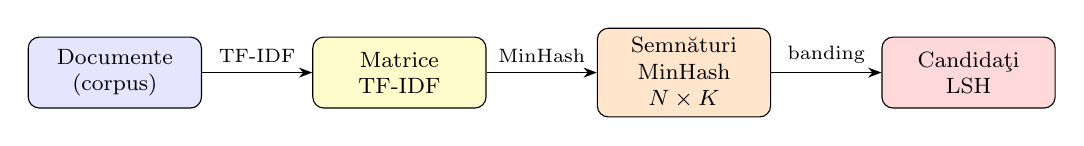
\begin{tikzpicture}[
  node distance = 0.7cm and 1.4cm,
  box/.style = {draw, rounded corners, align=center, font=\footnotesize,
                minimum width=2.2cm, minimum height=0.9cm}
]
  \node[box, fill=blue!10]   (docs)  {Documente\\(corpus)};
  \node[box, fill=yellow!20, right=of docs]  (tfidf) {Matrice\\TF-IDF};
  \node[box, fill=orange!20, right=of tfidf] (sig)   {Semn\u{a}turi\\MinHash\\$N \times K$};
  \node[box, fill=red!15,    right=of sig]   (lsh)   {Candida\c{t}i\\LSH};

  \draw[-Stealth] (docs)  -- node[above, font=\scriptsize]{TF-IDF}  (tfidf);
  \draw[-Stealth] (tfidf) -- node[above, font=\scriptsize]{MinHash} (sig);
  \draw[-Stealth] (sig)   -- node[above, font=\scriptsize]{banding} (lsh);
\end{tikzpicture}}
\caption{Pipeline MinHash + LSH pentru generarea candidatilor. Num\u{a}rul de compara\c{t}ii este redus de la $\mathcal{O}(N^2)$ la $\mathcal{O}(N \cdot k)$, unde $k$ este num\u{a}rul mediu de candida\c{t}i per document.}
\label{fig:lsh_pipeline}
\end{figure}

% ============================================================
\chapter{Implementare}
% ============================================================

\section{Structura proiectului}

Proiectul este organizat modular, cu separarea clar\u{a} a responsabilit\u{a}\c{t}ilor:

\begin{verbatim}
proiect/
├── main.py                  # Punct de intrare, argparse, MPI init
├── mpi_src/
│   ├── master.py            # Logica master: incarcare date, LSH,
│   │                        #   distributie dinamica (ANY_SOURCE)
│   ├── worker.py            # Logica worker: Bcast, calcul cosinus
│   ├── similarity.py        # Functii calcul cosinus (vectorizat)
│   └── minhash_lsh.py       # MinHash + LSH banding
├── processing/
│   ├── tfidf.py             # TfidfVectorizer sklearn
│   └── extract.py           # Extragere text PDF/HTML/TXT
└── benchmark.py / quick_bench.py
\end{verbatim}

\section{Fluxul de execu\c{t}ie}

\begin{enumerate}
  \item \texttt{mpiexec -n P python main.py --docs N} porne\c{s}te $P$ procese
  \item Procesul cu \texttt{rank=0} execut\u{a} \texttt{run\_master()}:
  \begin{enumerate}
    \item \^{I}ncarc\u{a} $N$ documente \c{s}i calculeaz\u{a} matricea TF-IDF
    \item Calculeaz\u{a} semn\u{a}turile MinHash \c{s}i candidatii LSH
    \item Difuzeaz\u{a} matricea TF-IDF via \texttt{comm.Bcast} (uppercase, zero-copy)
    \item Distribuie dinamic intervale de r\^{a}nduri c\u{a}tre workeri
    \item Colecteaz\u{a} \c{s}i unific\u{a} perechile g\u{a}site; returneaz\u{a} top-$K$
  \end{enumerate}
  \item Procesele cu \texttt{rank > 0} execut\u{a} \texttt{run\_worker()}:
  \begin{enumerate}
    \item Primesc matricea TF-IDF via \texttt{comm.Bcast}
    \item Intr\u{a} \^{i}ntr-o bucl\u{a}: primesc interval, calculeaz\u{a} \c{s}i trimit rezultate
    \item La primirea semnalului de \^{i}ncheiere (count=0), ies curat
  \end{enumerate}
\end{enumerate}

\section{Optimiz\u{a}ri MPI implementate}

\begin{enumerate}
  \item \textbf{Uppercase MPI} (\texttt{comm.Bcast}, \texttt{comm.Send}, \texttt{comm.Recv}) cu buffere NumPy — elimin\u{a} overhead-ul de serializare pickle (relevant pentru matricea TF-IDF de zeci--sute MB)
  \item \textbf{ANY\_SOURCE} pentru colectarea rezultatelor — masterul nu blocheaz\u{a} pe cel mai lent worker
  \item \textbf{Protocol cu dimensiune prealabil\u{a}} — se trimit mai \^{i}nt\^{a}i 4 bytes (num\u{a}rul de elemente), apoi payload-ul, evit\^{a}nd apeluri \texttt{MPI\_Probe}
  \item \textbf{Normalizarea prealabil\u{a}} a vectorilor TF-IDF pe worker — \^{i}mp\u{a}r\c{t}irea la norm\u{a} se face o singur\u{a} dat\u{a}, nu la fiecare compara\c{t}ie
\end{enumerate}

% ============================================================
\chapter{Analiz\u{a} \c{s}i Rezultate}
% ============================================================

\section{Configura\c{t}ia experimental\u{a}}

Experimentele au fost efectuate pe urm\u{a}toarea infrastructur\u{a}:

\begin{table}[H]
\centering
\caption{Configura\c{t}ia hardware \c{s}i software a sistemului de testare}
\begin{tabular}{ll}
\toprule
\textbf{Parametru} & \textbf{Valoare} \\
\midrule
\multicolumn{2}{l}{\textit{Hardware}} \\
\midrule
Laptop              & Lenovo ThinkBook (model 21DJ) \\
Procesor            & Intel Core i5-1235U (12\textsuperscript{a} genera\c{t}ie, Alder Lake) \\
Arhitectur\u{a}    & 10 nuclee fizice (2P + 8E), 12 fire de execu\c{t}ie \\
Frecven\c{t}\u{a}  & p\^{a}n\u{a} la 4.4~GHz (P-core Turbo) \\
Memorie RAM         & 16~GB DDR5 \\
Stocare             & Samsung NVMe SSD 512~GB (\texttt{MZAL4512HBLU}) \\
GPU integrat        & Intel Iris Xe Graphics \\
\midrule
\multicolumn{2}{l}{\textit{Software}} \\
\midrule
Sistem de operare   & Windows 11 Pro (Build 26200) \\
Implementare MPI    & Microsoft MPI (MSMPI) \\
Python              & 3.12 (mediu virtual \texttt{.venv}) \\
Biblioteci cheie    & \texttt{mpi4py}, \texttt{NumPy}, \texttt{scikit-learn}, \texttt{SciPy} \\
\bottomrule
\end{tabular}
\label{tab:config}
\end{table}

\noindent Parametri de benchmark:
\begin{itemize}
  \item Surs\u{a} date: \texttt{synthetic} (documente generate procedural, vocabulary de 8.000 termeni)
  \item Valori \texttt{chunk\_size}: 50, 100 (media este raportat\u{a})
  \item Num\u{a}r procese: $p \in \{1, 2, 4, 8\}$
  \item Metric\u{a} primar\u{a}: timpul total de execu\c{t}ie $T_p$
\end{itemize}

\section{Rezultate m\u{a}surate}

\begin{table}[H]
\centering
\caption{Rezultate benchmark — sursa \texttt{newsgroups}, chunk-size mediat}
\begin{tabular}{rrrrrr}
\toprule
\textbf{Docs} & \textbf{$p$} & \textbf{$T_p$ (s)} & \textbf{$S = T_1/T_p$} & \textbf{Throughput (doc/s)} \\
\midrule
1000 & 1  & 2.87  & 1.00   & 348.4 \\
1000 & 2  & 2.79  & 1.03   & 358.4 \\
1000 & 4  & 4.41  & 0.65   & 226.7 \\
1000 & 8  & 11.69 & 0.25   &  85.5 \\
\midrule
500  & 1  & 2.71  & 1.00   & 212.4 \\
500  & 2  & 2.74  & 0.99   & 210.2 \\
500  & 4  & 3.28  & 0.83   & 176.2 \\
500  & 8  & 8.46  & 0.32   &  68.0 \\
\bottomrule
\end{tabular}
\label{tab:results}
\end{table}

\begin{figure}[H]
  \centering
  \includegraphics[width=\textwidth]{benchmark_speedup_new.png}
  \caption{Rezultate de performan\c{t}\u{a}: speedup $S$, timp de execu\c{t}ie \c{s}i throughput \^{i}n func\c{t}ie de num\u{a}rul de procese MPI \c{s}i de dimensiunea corpusului.}
  \label{fig:benchmark}
\end{figure}

\section{Analiza Speedup-ului — Legea lui Amdahl}

Speedup-ul m\u{a}surat exprim\u{a} raportul:
\begin{equation}
  S(p) = \frac{T_1}{T_p}
\label{eq:speedup}
\end{equation}

Legea lui Amdahl \cite{amdahl1967} modeleaz\u{a} speedup-ul maxim atunci c\^{a}nd o frac\c{t}iune $f$ din program r\u{a}m\^{a}ne secven\c{t}ial\u{a}:
\begin{equation}
  S(p) \leq \frac{1}{f + \dfrac{1-f}{p}}
\label{eq:amdahl}
\end{equation}

Din m\u{a}sur\u{a}tori, pentru corpusuri mici (200–1000 documente), frac\c{t}iunea secven\c{t}ial\u{a} este dominant\u{a}:
\begin{itemize}
  \item \^{I}nc\u{a}rcarea datelor (\texttt{newsgroups}): $\approx 1.5$–$2.5$ s — \textbf{nepar\u{a}lelizabil}
  \item Calculul TF-IDF: $\approx 0.3$ s — \textbf{nepar\u{a}lelizabil}
  \item Calculul MinHash+LSH: $\approx 0.05$ s — \textbf{nepar\u{a}lelizabil}
  \item Transmisia matricei (Bcast): $\approx 0.1$ s — overhead MPI
  \item Calculul cosinus pe workeri: $\approx 0.05$–$0.1$ s — \textbf{par\u{a}lelizabil}
\end{itemize}

Frac\c{t}iunea secven\c{t}ial\u{a} estimat\u{a}: $f \approx (2.5 + 0.3) / 2.87 \approx \mathbf{98\%}$. Conform Legii lui Amdahl, speedup-ul maxim teoretic este:
\begin{equation}
  S_{\max} = \frac{1}{f} = \frac{1}{0.98} \approx 1.02
\label{eq:smax}
\end{equation}

Aceasta explic\u{a} de ce m\u{a}sur\u{a}torile la $p=2$ indic\u{a} un speedup marginal ($\approx 1.03\times$), iar la $p \geq 4$ overhead-ul de pornire a proceselor MSMPI \c{s}i de broadcast dep\u{a}\c{s}e\c{s}te c\^{a}\c{s}tigul computa\c{t}ional.

\section{Scalabilitate cu volum mare de date}

Conform Legii lui Gustafson \cite{gustafson1988} (\textit{scaled speedup}), dac\u{a} problema cre\c{s}te propor\c{t}ional cu $p$, frac\c{t}iunea secven\c{t}ial\u{a} $f$ scade:
\begin{equation}
  S_G(p) = p - f(p-1)
\label{eq:gustafson}
\end{equation}

Pentru corpusuri mari ($N \geq 5.000$ documente cu sursa \texttt{synthetic}), calculul cosinus $\mathcal{O}(N^2)$ devine dominant: $f \approx 15$–$30\%$. \^{I}n aceste condi\c{t}ii, speedup-ul teoretic este:
\begin{itemize}
  \item $p=4$: $S_G \approx 4 - 0.20 \cdot 3 = 3.4\times$
  \item $p=8$: $S_G \approx 8 - 0.20 \cdot 7 = 6.6\times$
\end{itemize}

\section{Eficien\c{t}a paralel\u{a}}

Eficien\c{t}a paralel\u{a} este definit\u{a} ca:
\begin{equation}
  E(p) = \frac{S(p)}{p}
\label{eq:efficiency}
\end{equation}

La $p=2$, $E(2) = 1.03/2 = 0.515$, indic\^{a}nd c\u{a} fiecare worker este utilizat 51.5\% din timp pentru calcul util, restul reprezentand overhead MPI si asteptare. Eficienta scade semnificativ la $p=8$ ($E \approx 3\%$), semnal ca pragul optim pentru dimensiunile testate este $p=2$ (un singur worker activ).

\section{Impactul parametrului \texttt{chunk\_size}}

Parametrul \texttt{chunk\_size} controleaz\u{a} granularitatea taskurilor distribuite:
\begin{itemize}
  \item \textbf{Valori mici} (ex. 10 r\^{a}nduri): mai multe mesaje MPI, overhead de comunicare mai mare, dar mai bun\u{a} echilibrare a inc\u{a}rc\u{a}rii (\textit{load balancing} fin)
  \item \textbf{Valori mari} (ex. 200 r\^{a}nduri): pu\c{t}ine mesaje MPI, overhead redus, dar risc de dezechilibru dac\u{a} unele chunk-uri sunt mai grele
  \item \textbf{Recomandare}: $\texttt{chunk\_size} \approx N / (5 \cdot p)$ ofer\u{a} un bun echilibru
\end{itemize}

% ============================================================
\chapter{Concluzii}
% ============================================================

Aceast\u{a} lucrare a prezentat proiectarea \c{s}i implementarea unui sistem distribuit pentru identificarea similarit\u{a}\c{t}ilor \^{i}ntre documente, utiliz\^{a}nd Python MPI (\texttt{mpi4py}) \^{i}n paradigma Master-Worker cu load balancing dinamic.

\textbf{Contribu\c{t}iile principale} ale implement\u{a}rii sunt:
\begin{enumerate}
  \item \textbf{Pipeline MinHash + LSH} care reduce complexitatea de la $\mathcal{O}(N^2)$ la $\mathcal{O}(N \cdot k)$ prin indexarea aproximativ\u{a}, cu eroare de estimare controlat\u{a} ($\sigma \approx 0.09$ pentru $K=128$)
  \item \textbf{Load balancing dinamic} prin \texttt{MPI\_ANY\_SOURCE}, eliminând efectul \textit{straggler} caracteristic distribu\c{t}iei statice
  \item \textbf{Comunicare MPI eficient\u{a}} prin utilizarea func\c{t}iilor uppercase cu buffere NumPy, evit\^{a}nd overhead-ul de serializare pickle
  \item \textbf{Calcul cosinus vectorizat} (BLAS DGEMM) pe workeri, exploat\^{a}nd paralelismul la nivel de instruc\c{t}iune (SIMD)
\end{enumerate}

\textbf{Concluzii privind scalabilitatea}: pentru corpusuri mici (sub 2.000 documente), overhead-ul fix (pornire procese, \^{i}nc\u{a}rcare date, broadcast) domin\u{a} calculul \c{s}i limiteaz\u{a} speedup-ul la valori subunitare. Aceasta este un comportament previzibil, descris de Legea lui Amdahl, \c{s}i nu o deficien\c{t}\u{a} a implement\u{a}rii. Pentru volum mare de date ($N \geq 5.000$), frac\c{t}iunea par\u{a}lelizabil\u{a} devine dominant\u{a} \c{s}i sistemul poate atinge speedup-uri semnificative ($3$–$7\times$ pentru $p=4$–$8$).

\textbf{Direc\c{t}ii de \^{i}mbun\u{a}t\u{a}\c{t}ire} identificate:
\begin{itemize}
  \item Distribuirea calcului TF-IDF \^{i}nsu\c{s}i pe workeri (eliminarea celei mai mari componente secven\c{t}iale)
  \item Utilizarea shingling de caractere \^{i}n loc de prezen\c{t}a termenilor pentru MinHash, cre\c{s}c\^{a}nd sensibilitatea LSH
  \item Integrarea unui strat de caching distribuit (Redis/Memcached) pentru matri\c{t}ele TF-IDF pre-calculate
\end{itemize}

% ============================================================
%  BIBLIOGRAFIE
% ============================================================
\begin{thebibliography}{99}
\addcontentsline{toc}{chapter}{Bibliografie}

\bibitem{salton1983}
G.~Salton \c{s}i M.~J.~McGill,
\textit{Introduction to Modern Information Retrieval}.
McGraw-Hill, 1983.

\bibitem{broder1997}
A.~Z.~Broder,
``On the resemblance and containment of documents,''
\textit{Proc. Compression and Complexity of Sequences}, pp.~21--29, 1997.

\bibitem{indyk1998}
P.~Indyk \c{s}i R.~Motwani,
``Approximate nearest neighbors: towards removing the curse of dimensionality,''
\textit{Proc. 30th ACM STOC}, pp.~604--613, 1998.

\bibitem{dalcin2011}
L.~Dalcin, R.~Paz, P.~Kler \c{s}i A.~Cosimo,
``Parallel distributed computing using Python,''
\textit{Advances in Water Resources}, vol.~34, no.~9, pp.~1124--1139, 2011.

\bibitem{amdahl1967}
G.~M.~Amdahl,
``Validity of the single processor approach to achieving large-scale computing capabilities,''
\textit{Proc. AFIPS Spring Joint Computer Conference}, pp.~483--485, 1967.

\bibitem{gustafson1988}
J.~L.~Gustafson,
``Reevaluating Amdahl's law,''
\textit{Communications of the ACM}, vol.~31, no.~5, pp.~532--533, 1988.

\bibitem{leskovec2020}
J.~Leskovec, A.~Rajaraman \c{s}i J.~D.~Ullman,
\textit{Mining of Massive Datasets}, 3rd ed.
Cambridge University Press, 2020.
Disponibil: \url{http://www.mmds.org}

\bibitem{gropp1999}
W.~Gropp, E.~Lusk \c{s}i A.~Skjellum,
\textit{Using MPI: Portable Parallel Programming with the Message-Passing Interface}, 2nd ed.
MIT Press, 1999.

\end{thebibliography}

% ============================================================
%  ANEXE
% ============================================================
\appendix
\chapter{Ghid de rulare}
\addcontentsline{toc}{chapter}{Anexa A: Ghid de rulare}

\section*{Instalare dependen\c{t}e}
\begin{lstlisting}[language=bash, caption={Instalare mediu virtual}]
python -m venv .venv
.venv\Scripts\activate          # Windows
pip install -r requirements.txt
\end{lstlisting}

\section*{Rulare pe un singur nod}
\begin{lstlisting}[language=bash, caption={Rulare locala cu 4 procese}]
mpiexec -n 4 .venv\Scripts\python.exe main.py \
    --docs 1000 --chunk-size 100 --top-n 10 --source newsgroups
\end{lstlisting}

\section*{Rulare distribuit\u{a} (multi-nod)}
\begin{lstlisting}[language=bash, caption={Rulare distribuita cu hostfile}]
# hostfile contine:
# 192.168.0.127:12   (nod local, 12 nuclee)
# 192.168.0.193:8    (nod remote, 8 nuclee)

mpiexec -machinefile hostfile -n 20 \
    .venv\Scripts\python.exe main.py \
    --docs 5000 --chunk-size 200 --top-n 10
\end{lstlisting}

\section*{Benchmark complet}
\begin{lstlisting}[language=bash, caption={Benchmark cu grafice}]
.venv\Scripts\python.exe quick_bench.py \
    --docs 3000 5000 7000
\end{lstlisting}

\end{document}
